% Compile twice with LuaLaTeX from this directory.
\documentclass[a4paper,11pt]{ltjsarticle}
\usepackage[top=19mm,bottom=19mm,left=20mm,right=20mm,headheight=16pt,headsep=6mm]{geometry}
\usepackage{luatexja-fontspec}
\setmainfont[Path=C:/Windows/Fonts/,BoldFont=timesbd.ttf,ItalicFont=timesi.ttf,BoldItalicFont=timesbi.ttf]{times.ttf}
\setsansfont[Path=C:/Windows/Fonts/,BoldFont=arialbd.ttf]{arial.ttf}
\setmainjfont[Path=C:/Windows/Fonts/,BoldFont=yumindb.ttf]{yumin.ttf}
\setsansjfont[Path=C:/Windows/Fonts/,BoldFont=YuGothB.ttc]{YuGothM.ttc}
\usepackage{amsmath,amssymb,graphicx,booktabs,tabularx,array}
\usepackage{xcolor,tikz,tcolorbox,fancyhdr,enumitem}
\usetikzlibrary{arrows.meta,positioning,calc,fit,backgrounds}
\definecolor{navy}{HTML}{203C55}
\definecolor{teal}{HTML}{138B86}
\definecolor{orange}{HTML}{D77932}
\definecolor{pale}{HTML}{F0F6F7}
\definecolor{muted}{HTML}{657987}
\definecolor{light}{HTML}{D6E1E5}
\usepackage[unicode,colorlinks=true,linkcolor=teal,urlcolor=teal,citecolor=teal]{hyperref}
\hypersetup{pdftitle={グラフの構造からCIMのよい種を考える},pdfauthor={研究調査資料},pdfsubject={G22・G55・G70の構造比較と先行研究}}
\graphicspath{{figures/}}
\pagestyle{fancy}\fancyhf{}
\fancyhead[L]{\small\sffamily\color{muted}グラフ構造・Max-Cut・CIM}
\fancyhead[R]{\small\sffamily\color{muted}研究レビュー / 2026.09.21}
\fancyfoot[L]{\footnotesize\color{muted}構造の実測と文献調査}
\fancyfoot[R]{\sffamily\color{navy}\thepage}
\renewcommand{\headrulewidth}{0.3pt}
\setlength{\parindent}{1em}\setlength{\parskip}{3pt}
\renewcommand{\baselinestretch}{0.99}
\renewenvironment{center}{\par\vspace{2pt}\centering}{\par\vspace{2pt}}
\setlist[itemize]{leftmargin=1.5em,itemsep=3pt,topsep=4pt}
\setlist[enumerate]{leftmargin=1.8em,itemsep=4pt,topsep=4pt}
\newcommand{\pagehead}[3]{\noindent{\sffamily\small\color{teal}#1}\par\vspace{1mm}\noindent{\sffamily\bfseries\LARGE\color{navy}#2}\par\vspace{1mm}\noindent{\color{muted}#3}\par\vspace{2mm}}
\newcommand{\sub}[1]{\par\vspace{2mm}\noindent{\sffamily\bfseries\large\color{navy}#1}\par}
\newcommand{\figcap}[2]{\par\vspace{1mm}\noindent{\small\sffamily\color{teal}図#1}\quad{\small #2}\par\vspace{2mm}}
\newcommand{\source}[1]{\par\noindent{\footnotesize\color{muted}出典・根拠：#1}\par}
\newtcolorbox{point}[1]{colback=pale,colframe=teal,boxrule=.5pt,arc=1.5mm,left=3mm,right=3mm,top=2mm,bottom=2mm,title=#1,coltitle=white,fonttitle=\sffamily\bfseries}
\newtcolorbox{caution}[1]{colback=orange!5,colframe=orange!70,boxrule=.4pt,arc=1.5mm,left=3mm,right=3mm,top=2mm,bottom=2mm,title=#1,coltitle=navy,colbacktitle=orange!16,fonttitle=\sffamily\bfseries}
\tikzset{box/.style={draw=light,fill=pale,rounded corners=2mm,align=center,font=\sffamily\small,text=navy,minimum height=14mm,text width=32mm,inner sep=3mm},flow/.style={-{Stealth[length=2.5mm]},thick,draw=teal},dot/.style={circle,fill=teal,inner sep=0pt,minimum size=4mm}}
\begin{document}
\thispagestyle{empty}
\noindent{\sffamily\bfseries\color{teal}\large RESEARCH NOTE}\hfill{\sffamily\color{muted}2026年9月21日}
\vspace{12mm}

\noindent{\sffamily\bfseries\fontsize{29}{40}\selectfont\color{navy}グラフの構造から\\CIMの「よい種」を考える}\par
\vspace{5mm}
\noindent{\sffamily\Large G22・G55・G70の結合構造と先行研究}\par
\vspace{5mm}
\noindent\color{teal}\rule{\textwidth}{1.2pt}\color{black}
\vspace{5mm}

同じMax-Cutでも、グラフによって探索の進み方は変わる。頂点の数だけでは見えない「つながり方」を調べると、CIMで得た解をGAやSAに渡す際に、何を評価すべきかが見えてくる。

本資料は、まず\textbf{入力グラフそのものの構造}を理解し、その知識を\textbf{将来よい解に育つ候補の選別}へつなぐためのレビューである。グラフを扱うTransformerの先行研究も、この流れの中に位置づける。

\vspace{5mm}
\begin{center}
\begin{tikzpicture}
\node[box,text width=35mm,minimum height=23mm] (a) {\textbf{構造を知る}\\橋・core・固有値};
\node[box,text width=35mm,minimum height=23mm,right=8mm of a] (b) {\textbf{解の配置を見る}\\どの辺を切れているか};
\node[box,text width=35mm,minimum height=23mm,right=8mm of b] (c) {\textbf{種の価値を予測}\\GA / SAでの到達品質};
\draw[flow] (a)--(b);\draw[flow] (b)--(c);
\end{tikzpicture}
\end{center}
\figcap{1}{研究の見取り図。左側の構造評価が今回の主題。右側は、それを候補解の選別へ発展させる研究案である。}

\begin{point}{今回の実測で見えたこと}
G70は10,000頂点あるが、最大二重連結ブロックは4,798頂点。G55の4,789頂点とほぼ同じ大きさだった。一方、G70には3,605本の橋があり、G22には橋も関節点もない。\textbf{元の大きさと、分解した後の構造は分けて見る必要がある。}
\end{point}

\sub{この資料の読み方}
2--3ページで用語を図解し、4--5ページで実測結果と評価指標を読む。6--7ページは先行研究、8--9ページは候補評価と実験の設計、10ページは参考文献と再現情報である。

\vfill
\noindent{\small\color{muted}対象：リポジトリ内のG22・G55・G70。確認HEAD：9053ca4（2026年9月14日）。\\本資料の構造値は実測値。模式図と研究案は明示して区別した。学習モデルの性能実験は未実施。}

\newpage
\pagehead{01 / 基本の整理}{グラフと解は、何が違うのか}{「結合性」を評価する対象を、最初にそろえる。}

\sub{グラフは問題、解はその上の割当て}
グラフ$G=(V,E)$は、頂点の集合$V$と、それを結ぶ辺の集合$E$からなる。今回の入力では全辺の重みが$+1$である。Max-Cutは頂点を二つの組に分け、\textbf{異なる組を結ぶ辺の本数}をできるだけ大きくする問題だ。

一つの解$s$は、各頂点をどちらの組に入れるかという割当てである。グラフが同じでも、割当てが変わればcut値は変わる。

\begin{center}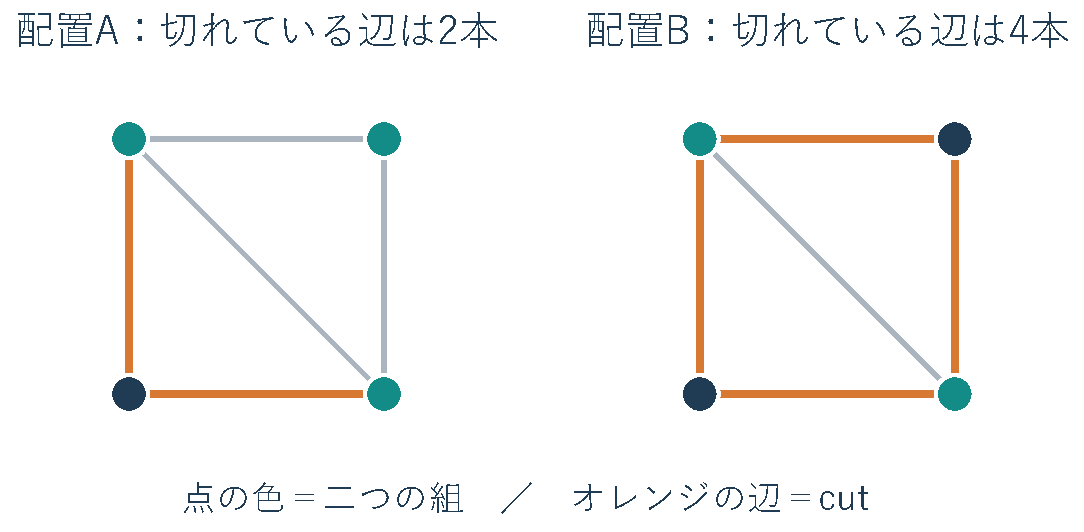
\includegraphics[height=48mm]{cut_example.pdf}\end{center}
\figcap{2}{同じグラフに対する二つの解。点の色は割当て、オレンジの辺は異なる色の点を結ぶ辺。配置Bは4本をcutしている。説明用の小さなグラフであり、G-setの実データではない。}

\sub{式で書くと、何を数えているかが分かる}
頂点$i$の割当てを$s_i\in\{-1,+1\}$とすると、cut値は次で表せる。
\[
 C_G(s)=\sum_{\{i,j\}\in E}w_{ij}\frac{1-s_is_j}{2}
\]
異なる組なら$s_is_j=-1$なので、その辺は重み$w_{ij}$だけ加点される。同じ組なら加点は0である。したがって、全頂点の符号を同時に反転してもcut値は変わらない。

\begin{point}{グラフを評価することと、候補を評価すること}
構造の特徴$\phi(G)$は「この問題はどのようなつながり方をしているか」を表す。同じグラフから作ったCIM解には、同じ$\phi(G)$が対応する。候補間の順位をつける段階では、割当て$s$を加えた$f(G,s)$が必要になる。
\end{point}

\sub{CIM・GA・SAの役割}
CIMはCoherent Ising Machineの略で、ここではMax-Cutの候補解を生成する役割を想定する。GAは集団内の交叉や変異、SAは温度に応じた状態遷移によって、渡された候補からさらによい解を探す。

欲しいのは「いまcutが大きい解」だけでなく、\textbf{後段の探索に使ったときにも有利な解}である。構造を調べる理由は、その違いを説明する材料を得ることにある。

\newpage
\pagehead{02 / 構造の図解}{「つながっている」の中身を分ける}{橋・関節点・coreを使うと、見かけの大きさを分解できる。}

\begin{center}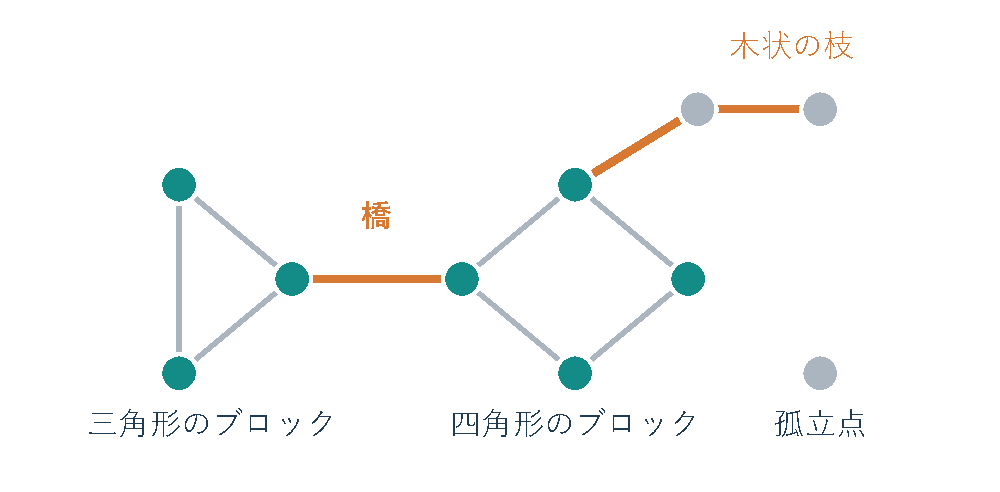
\includegraphics[height=48mm]{decomposition.pdf}\end{center}
\figcap{3}{構造の模式図。オレンジの辺は橋。二つの閉路の間や木状の枝にある辺は、1本除くだけでグラフが分断される。離れた点は孤立点である。}

\noindent\begin{tabularx}{\textwidth}{@{}p{29mm}X@{}}
\toprule
\textbf{指標・用語} & \textbf{何を見ているか}\\\midrule
連結成分 & 辺をたどって行き来できる頂点のまとまり。孤立点も1成分と数える。\\
橋・関節点 & その辺、またはその頂点を除くと分断される場所。構造上の接続の弱い箇所を表す。\\
二重連結ブロック & 関節点で分けた部分。Max-Cutでは各ブロックを独立に解き、割当ての向きを合わせて結合できる。[2]\\
core number & 頂点がどの程度の最小次数を持つ部分グラフに残れるか。局所的な結合の厚みを表す。\\\bottomrule
\end{tabularx}

\sub{2-coreは、孤立点と葉を繰り返し除いた残り}
次数とは、その頂点につながる辺の本数である。次数0の頂点と次数1の頂点を除くと、別の頂点が新たに次数1になることがある。これを止まるまで続けると2-coreが残る。

\begin{center}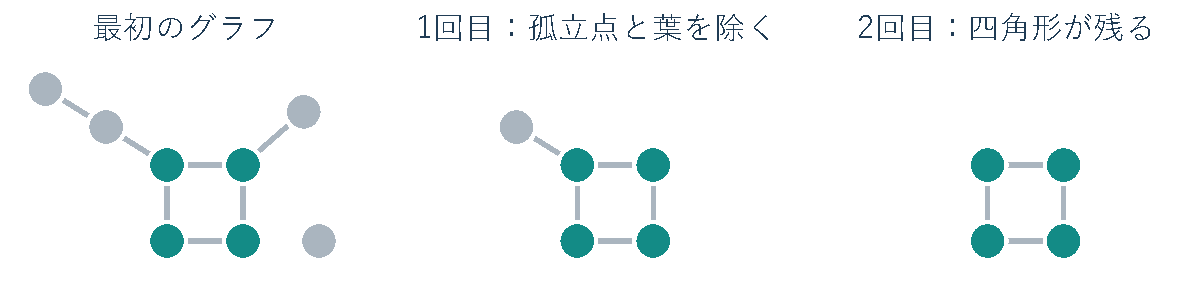
\includegraphics[height=36mm]{core_peeling.pdf}\end{center}
\figcap{4}{2-coreの作り方。最初に枝の先端と孤立点が消え、次に残った枝が消える。この例では四角形が残る。一般に2-coreと二重連結ブロックは同じ概念ではない。}

\begin{point}{なぜMax-Cutと関係があるのか}
正重みの橋は、片側の頂点の割当てを丸ごと反転すれば、ほかの辺のcut状態を変えずにcutできる。したがって、\textbf{橋や木状部分と、閉路を含む主要部分を分けて評価する}ことに意味がある。ただし、現行GA/SAの探索過程まで同じになるわけではない。
\end{point}
\source{構造分解のMax-Cutへの利用はRehfeldtほか[2]。図3・4は説明用に作成。}

\newpage
\pagehead{03 / 入力の実測}{G70は「1万頂点」だけでは語れない}{同じ方法で3グラフを測り、構造の違いを比較した。}

\noindent\begin{tabularx}{\textwidth}{@{}Xrrr@{}}
\toprule
\textbf{指標} & \textbf{G22} & \textbf{G55} & \textbf{G70}\\\midrule
頂点数 / 辺数 & 2,000 / 19,990 & 5,000 / 12,498 & 10,000 / 9,999\\
平均次数 & 19.9900 & 4.9992 & 1.9998\\
連結成分数（孤立点を含む） & 1 & 32 & 1,598\\
孤立点 & 0 & 31 & 1,354\\
橋 / 関節点 & 0 / 0 & 180 / 179 & 3,605 / 2,770\\
最大二重連結ブロックの頂点数 & 2,000 & 4,789 & 4,798\\
2-core内の辺数 & 19,990 & 12,318 & 6,394\\
最大core number & 14 & 3 & 2\\\bottomrule
\end{tabularx}

\vspace{3mm}
\begin{center}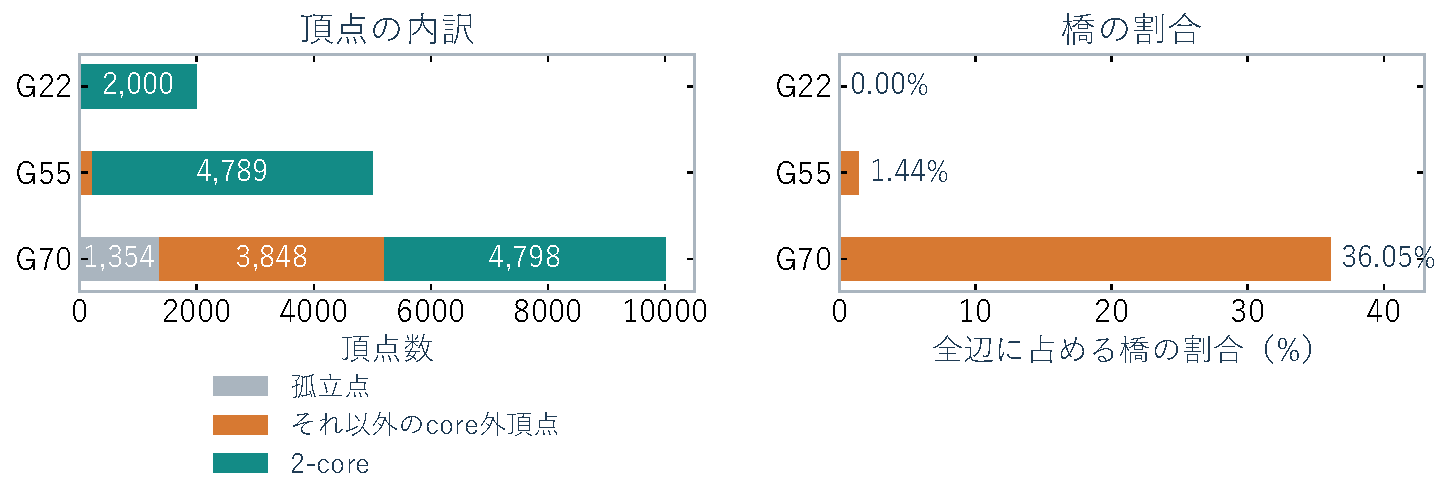
\includegraphics[width=\textwidth,height=67mm,keepaspectratio]{comparison.pdf}\end{center}
\figcap{5}{左は頂点の内訳、右は橋の割合。G70の2-coreは全頂点の47.98\%で、全辺の約36.05\%が橋である。左図のオレンジは孤立点以外で2-coreに残らない頂点を表す。}

\sub{この比較から読めること}
G22は全体が一つの二重連結ブロックで、橋や関節点では分けられない。G55とG70は元の頂点数が2倍違うが、最大ブロックの頂点数はほぼ同じである。一方、2-core内の辺数はG55がG70の約1.93倍あり、同じ規模でも結合の密さが異なる。

このため、グラフの比較には\textbf{元の頂点数、主要部の大きさ、主要部の密さ}を一緒に使うのが自然である。この3指標だけで、CIMやGA/SAの成績の順序が決まると結論づけることはできない。

\begin{caution}{実測と原因の推定は分ける}
G70に橋や孤立点が多いことは確認できた。しかし、それが既存のGA実験での停滞を引き起こしたかは未検証である。主要ブロック内の解の違いと、後段探索の成績を照合する必要がある。
\end{caution}
\source{リポジトリ内の入力ファイルをNetworkX 3.6.1で集計。連結成分の基本集計は独立なBFS実装と一致。再現情報は10ページ。}

\newpage
\pagehead{04 / 指標の選び方}{密さと「切り分けやすさ」を見る}{平均次数・core・閉路・固有値は、それぞれ違う面を表す。}

\begin{center}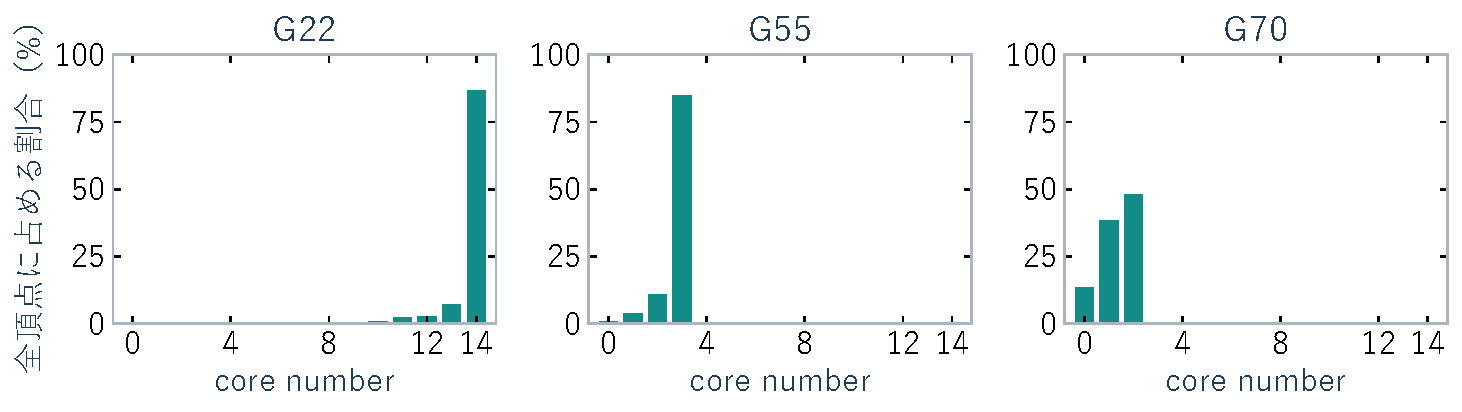
\includegraphics[height=45mm]{core_distribution.pdf}\end{center}
\figcap{6}{実測したcore numberの分布。G22では多くの頂点が14-coreに属する。一方、G70の最大core numberは2。横軸と縦軸を共通にして比較した。}

coreは、平均次数だけでは見えない局所的な結合を表す。ただし、core numberが大きいほど、常にMax-Cutや特定の探索法が難しくなるわけではない。最終的には性能データとの対応を確かめる。

\sub{奇数長の閉路には、切れない辺が必ず残る}
全辺が正重みのとき、偶数長の閉路は交互に二色を割り当てて全辺をcutできる。奇数長では一周したところで矛盾し、少なくとも1本が残る。

\begin{center}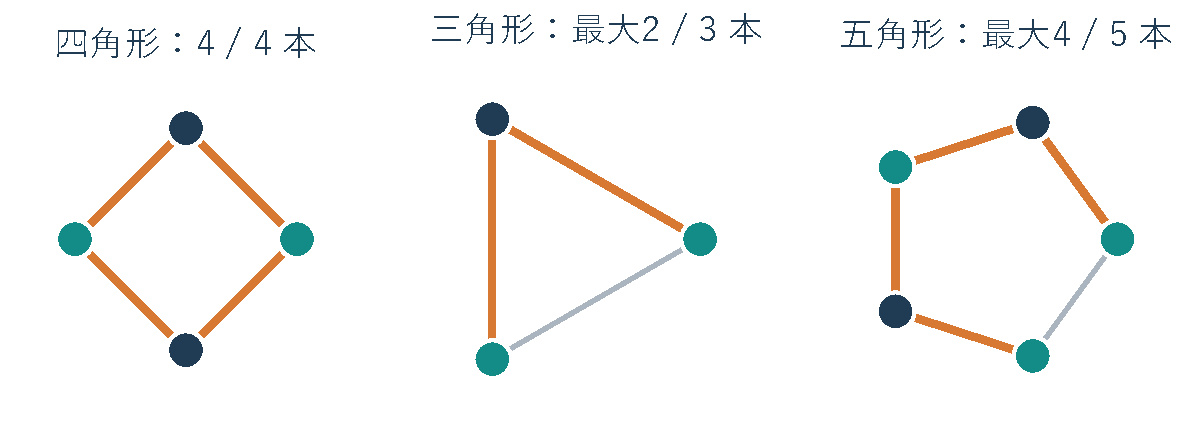
\includegraphics[height=40mm]{cycles.pdf}\end{center}
\figcap{7}{閉路とcutの模式図。G70の三角形数は0だが、二部グラフではないことを確認した。三角形数が0でも、五角形のような長い奇数閉路はあり得る。}

\sub{固有値は、どの行列・どの部分を見るかが大切}
固有値は、グラフの接続行列が持つ大域的なパターンを数値化する手段である。ラプラシアンの第2固有値は分断されにくさと関係する。一方、正規化隣接行列の下端の固有値は二部性と関係し、Max-Cutのスペクトル法に接点がある。[3]

\begin{point}{今回の指標候補}
まず\textbf{橋・関節点・ブロック・core分布}を使う。次に、最大連結成分や主要ブロック内の\textbf{連結性と二部性に関係する固有値}を追加する。G55/G70は非連結なので、全体の第2ラプラシアン固有値は0となり、それだけでは違いを捉えられない。
\end{point}
\source{core分布・三角形数は実測。スペクトルとMax-Cutの接点はTrevisan[3]。固有値そのものの数値計算は今回の集計には含めていない。}

\newpage
\pagehead{05 / 構造評価の先行研究}{最初に読むなら、MQLibから}{構造を測る研究と、それを探索性能へ結ぶ研究を整理する。}

\begin{center}
\begin{tikzpicture}
\node[box,text width=34mm] (g) {入力グラフ\\$G$};
\node[box,text width=39mm,right=8mm of g] (f) {構造の特徴量\\次数・core・固有値など};
\node[box,text width=36mm,right=8mm of f] (p) {予測モデル\\適した探索法を選ぶ};
\draw[flow] (g)--(f);\draw[flow] (f)--(p);
\end{tikzpicture}
\end{center}
\figcap{8}{MQLibの研究を今回の目的に沿って簡略化した図。グラフの特徴から探索法を選ぶ発想が、CIM・GA・SAの相性を調べる出発点になる。}

\sub{1. MQLib：構造から、何が得意かを予測する}
Dunning・Gupta・Silberholz（2018）は、多数のMax-Cut/QUBOヒューリスティックを比較し、問題の特徴から探索法を選ぶ仕組みを提供する。[1] 公開特徴量には、次数、クラスタリング係数、次数相関、core、重み、固有値関連の情報がある。

今回なら、「G22/G55/G70のどの特徴が、CIMや後段探索の成績差と関係するか」を調べる基準になる。ただし、\textbf{適したアルゴリズムを選ぶ問題と、同じグラフ内の候補を選ぶ問題は異なる。}

\sub{2. Rehfeldtほか：独立に解ける部分へ分ける}
Rehfeldt・Koch・Shinano（2023）は、疎なMax-Cut/QUBOの厳密解法を研究する。[2] 連結成分や二重連結成分への分解は、今回測った橋・関節点・最大ブロックに直接つながる。主要部の大きさを測る数学的な理由を与えるが、GA/SAの品質を予測する論文ではない。

\sub{3. Trevisan：固有値からMax-Cutを見る}
Trevisan（2009）は、最小固有値を使うMax-Cut近似法を示す。[3] 「よくつながっているか」だけでなく「二つの組に分けて辺を切りやすいか」を構造的に考えるための文献である。固有値とCIMの挙動の関係は、別途実験で検証する必要がある。

\sub{4. Schwartzman：部分グラフの疎さも重要}
Schwartzman（2024）は、arboricityを使って局所探索FLIPの平滑化計算量を解析する。[4] Arboricityは辺をいくつの森に分けられるかを表し、局所的な密さと関係する。core numberと同じ指標ではないが、平均次数だけでなく密な部分にも注目する背景になる。

\begin{caution}{理論の適用範囲}
[4]は重みの確率的摂動を仮定した計算量の結果である。今回の全重み$+1$のG-setや、GA/SAの到達品質の保証としては使えない。今回の特徴量候補は、これらの文献を踏まえた設計案である。
\end{caution}

\newpage
\pagehead{06 / 学習モデルの先行研究}{Transformerは、どこに使えるか}{グラフの表現、探索方策、将来価値を区別して読む。}

\begin{center}
\begin{tikzpicture}[node distance=7mm]
\node[box,text width=43mm] (s) {構造の情報\\辺・次数・core・位置情報};
\node[box,text width=43mm,below=7mm of s] (x) {候補解の情報\\割当て・cutされた辺};
\node[box,text width=38mm,minimum height=30mm] (m) at (6.9,-1.15) {グラフを扱うモデル\\MPNN / Transformer};
\node[box,text width=27mm,right=10mm of m,minimum height=30mm] (o) {出力\\候補の評価値};
\draw[flow] (s.east)--(m.west);\draw[flow] (x.east)--(m.west);\draw[flow] (m)--(o);
\end{tikzpicture}
\end{center}
\figcap{9}{今回考えられる評価器の概念図。これは提案する構成であり、下記の論文がそのまま実証したモデルではない。}

\sub{GraphGPS（NeurIPS 2022）：構造をどう入力するか}
GraphGPSは、位置・構造の符号化、近隣との情報交換、global attentionを組み合わせる。[5] ノードの並び順だけでなく、グラフ内の位置や関係を伝える方法を考える基盤になる。

今回への応用では、coreやブロックの所属などを入力へ加え、手設計の特徴量では失われる配置情報を学習させる。GraphGPS自体がCIMの種の選別を検証したわけではない。

\sub{MARCO（IJCAI 2024）：TransformerでMax-Cutを探索する}
MARCOはGraph Transformerを用い、辺の構造情報、現在の解、探索履歴を使って探索方策を学習する。[6] \textbf{TransformerをMax-Cutに使う具体例}として、まず読む価値がある。

ただし出力は探索の行動に関係するもので、既存GA/SAへ渡す種の評価値ではない。今回の目的へ転用するなら、予測対象と学習データを変更する必要がある。

\sub{ECO-DQN（AAAI 2020）：今後の報酬を予測する}
ECO-DQNはMPNNを使い、Max-Cutの状態に対する頂点反転の将来報酬を学習する。[7] MPNNとは、辺で結ばれた頂点間で情報を交換するニューラルネットワークである。「現在のcutを超えて将来を見る」という点が、候補評価の設計に近い。

\begin{point}{G70へ適用する際の計算量}
10,000頂点の全点attentionは、1ヘッドあたり$10^8$組の関係を扱う。大量候補を採点するなら推論費用も重要になる。GraphGPSの効率的attentionを使う構成や、疎なMPNNを比較対象にする。GraphGPSのすべての設定が線形計算量という意味ではない。
\end{point}

\newpage
\pagehead{07 / 評価関数の設計}{「いま良い」と「後で良くなる」を分ける}{グラフ構造を、候補解の将来価値へつなげる。}

\begin{center}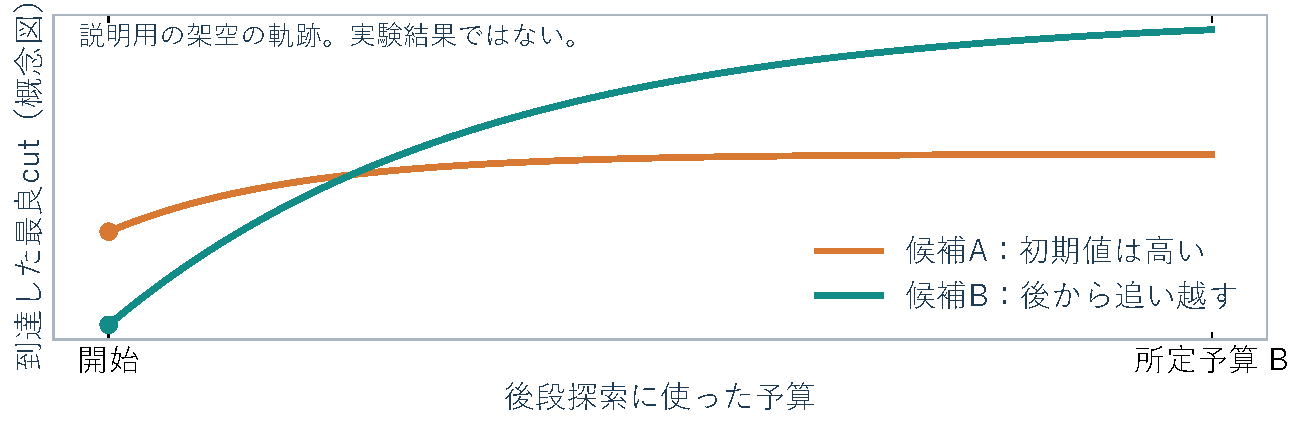
\includegraphics[width=.94\textwidth]{future_value.pdf}\end{center}
\figcap{10}{種の評価が目指すものを示した架空の例。初期cutが高い候補Aよりも、所定予算後は候補Bの方がよい。このような順位を事前に予測できるかを検証する。}

\sub{SAなら、初期解からの到達品質を教師にする}
SAの温度スケジュールや予算$B$を固定し、初期解$s$から到達する最良cutの期待値を考える。
\[
V_{\mathrm{SA}}(G,s;B)
=\mathbb{E}\!\left[\max_{0\leq t\leq B}C_G(s_t)\,\middle|\,s_0=s\right]
\]
複数の乱数系列で後段探索を実行し、この値や目標cutへの到達率を学習する。\textbf{改善量だけ}を教師にすると、初期値が低く伸びしろの大きい候補を優先してしまう場合がある。

\sub{GAなら、集団との相性も含める}
同じ候補でも、交叉相手や既存集団によって貢献は変わる。候補$s$を集団$P$へ追加・置換したときの結果を、$V_{\mathrm{GA}}(G,s,P;B)$として測る設計が考えられる。「候補単独の優秀さ」と「集団への貢献」は分けて検証する。

\noindent\begin{tabularx}{\textwidth}{@{}p{43mm}X@{}}
\toprule\textbf{候補ごとに測る量} & \textbf{構造と結びつける意味}\\\midrule
主要ブロック内のcut & 分解しやすい部分の得点と、主要部での得点を分ける。\\
未cut辺の集まり方 & 悪い辺が局所的に集中しているか、広く散っているかを見る。\\
頂点反転gainの分布 & すぐ改善できる頂点や、局所的に安定した配置を調べる。\\
辺のcut状態の違い & 孤立点の違いで、見かけの多様性が増える影響を避けやすい。\\\bottomrule
\end{tabularx}

\begin{caution}{これらは評価関数の候補であり、性能は未検証}
孤立点や連結成分全体の反転はcut状態を変えない。しかし、GA実装の交叉が同じ挙動になるとは限らない。目的関数の対称性と探索アルゴリズムの挙動を混同しない。
\end{caution}

\newpage
\pagehead{08 / 実験の組み立て}{選別によって、探索が良くなるか}{予測精度だけでなく、最終品質と総時間を同じ予算で比較する。}

\begin{center}
\begin{tikzpicture}
\node[box,text width=33mm] (a) {\textbf{1. 候補を集める}\\CIMを複数条件で実行};
\node[box,text width=33mm,right=8mm of a] (b) {\textbf{2. 教師を作る}\\固定予算のGA / SA};
\node[box,text width=33mm,right=8mm of b] (c) {\textbf{3. 評価器を学習}\\構造＋候補を入力};
\node[box,text width=33mm,below=12mm of c] (d) {\textbf{4. 未使用例で選別}\\上位候補を後段へ};
\node[box,text width=78mm,left=8mm of d] (e) {\textbf{5. 最終成績と総時間を比較}\\選別なし・cut順・多様性を使う方法とも比較};
\draw[flow](a)--(b);\draw[flow](b)--(c);\draw[flow](c)--(d);\draw[flow](d)--(e);
\end{tikzpicture}
\end{center}
\figcap{11}{提案する検証の流れ。候補を選ぶモデルの精度だけでなく、GA/SAの到達品質が実際に改善するかを評価する。}

\sub{最初の比較は、解釈しやすいモデルから}
まず構造と候補の明示的な特徴量に、小さな回帰・ランキングモデルを組み合わせる。次にMPNN、Graph Transformerへ進み、精度と推論時間の両方を比べる。初期cutをそろえた候補同士の比較を入れると、構造情報が初期cut以上の価値を持つかを調べやすい。

\sub{学習用と評価用は、グラフ単位でも分ける}
G22・G55・G70から何万個の解を生成しても、グラフ自体の例数は3である。同じ問題内の候補選別には使えるが、未知のグラフにも通用すると主張するには不十分だ。別のG-setや生成グラフを追加し、グラフごとに学習用と評価用を分ける。

\begin{point}{評価で必ず並べたい三つの値}
\textbf{最終品質}：所定予算後の最良cutや目標到達率。\\
\textbf{選別の効果}：無作為選択・初期cut順より良くなるか。\\
\textbf{総時間}：CIM生成、特徴計算、推論、後段探索を合計する。
\end{point}

学習用データを作る費用とモデルの訓練費用は、運用時の時間とは別に報告する。グラフだけに依存する特徴量は再利用できるが、候補$s$を含む計算は候補ごとに必要になる。

\sub{この研究で検証したい問い}
\begin{enumerate}
\item 橋・core・主要ブロックの構造は、CIMと後段探索の性能差を説明するか。
\item 同じ初期cutでも、構造上の配置を使うと「よい種」を選べるか。
\item Transformerの追加費用に見合う、最終品質や時間の改善が得られるか。
\end{enumerate}

\newpage
\pagehead{09 / 参考文献と再現情報}{読む順番と、確認した範囲}{まず[1]と[2]、Transformerに進むなら[6]と[5]を読む。}

{\small
\noindent\textbf{[1] Dunning, I.; Gupta, S.; Silberholz, J. (2018).}\\
\textit{What Works Best When? A Systematic Evaluation of Heuristics for Max-Cut and QUBO.} INFORMS Journal on Computing, 30(3), 608--624.\\
\href{https://github.com/MQLib/MQLib}{著者の公式実装・論文へのリンク} / \href{https://raw.githubusercontent.com/MQLib/MQLib/master/data/metrics.csv}{公開特徴量CSV}。
本資料では公式実装の説明と特徴量CSVを確認。論文PDF本文は未精読。

\noindent\textbf{[2] Rehfeldt, D.; Koch, T.; Shinano, Y. (2023).}\\
\textit{Faster exact solution of sparse MaxCut and QUBO problems.} Mathematical Programming Computation, 15, 445--470.\\
\href{https://link.springer.com/article/10.1007/s12532-023-00236-6}{公開全文・DOI: 10.1007/s12532-023-00236-6}。特にSection 4.1の分解。

\noindent\textbf{[3] Trevisan, L. (2009; preprint 2008).}\\
\textit{Max Cut and the Smallest Eigenvalue.} STOC 2009.\\
\href{https://arxiv.org/abs/0806.1978}{著者プレプリント: arXiv:0806.1978}。

\noindent\textbf{[4] Schwartzman, G. (2024).}\\
\textit{Local Max-Cut on Sparse Graphs.} ESA 2024, LIPIcs 308, Article 98.\\
\href{https://drops.dagstuhl.de/entities/document/10.4230/LIPIcs.ESA.2024.98}{論文・公開PDF: DOI 10.4230/LIPIcs.ESA.2024.98}。

\noindent\textbf{[5] Rampášek, L. et al. (2022).}\\
\textit{Recipe for a General, Powerful, Scalable Graph Transformer.} NeurIPS 2022.\\
\href{https://arxiv.org/abs/2205.12454}{論文: arXiv:2205.12454}。

\noindent\textbf{[6] Garmendia, A. I.; Cappart, Q.; Ceberio, J.; Mendiburu, A. (2024).}\\
\textit{MARCO: A Memory-Augmented Reinforcement Framework for Combinatorial Optimization.} IJCAI 2024, 6931--6939.\\
\href{https://www.ijcai.org/proceedings/2024/0766.pdf}{公開本文PDF} / \href{https://github.com/TheLeprechaun25/MARCO}{公式実装}。モデル構造はSection 5。

\noindent\textbf{[7] Barrett, T. D.; Clements, W. R.; Foerster, J. N.; Lvovsky, A. I. (2020).}\\
\textit{Exploratory Combinatorial Optimization with Reinforcement Learning.} AAAI 2020.\\
\href{https://ojs.aaai.org/index.php/AAAI/article/view/5723}{論文ページ・本文へのリンク}。
}

\sub{実測値の再現}
{\small
入力は\texttt{input/G22.txt}, \texttt{G55.txt}, \texttt{G70.txt}。宣言された全頂点を含め、自己ループ・重複辺がないことを確認した。集計の再実行は、リポジトリルートで次を実行する。
\begin{center}\texttt{python scripts/utils/graph\_structure\_audit.py}\end{center}
元の集計結果は\texttt{results/2026-09-21/graph\_connectivity/}内の\texttt{v2\_structure\_G22\_G55\_G70/summary.json}に保存され、入力のSHA256も含む。連結成分の基本値は独立BFS集計と一致した。図5・6はこのJSONから作成し、そのほかの図は説明用の模式図として作成した。
}

\begin{caution}{このレビューの到達点}
構造指標と関連研究の接点を整理した段階であり、提案した評価器の有効性は未検証である。CIM候補をTransformerで採点してGA/SAの種を選別する構成そのものの実証は、今回確認した範囲では見つからなかった。未発見を新規性の証明とは扱わない。
\end{caution}
\end{document}
